\documentclass{beamer}
\usepackage{beamerthemeshadow}
\usepackage{graphicx}
\usepackage{color}
\usepackage[utf8]{inputenc}
\usepackage{hyperref}
\usepackage[flushleft]{threeparttable}
\definecolor{}{rgb}{0.5, 0.3, 0.6}
\setbeamercolor{structure}{}

\usepackage[T2A]{fontenc}



\def\d{{\fontencoding{T1}\selectfont\dj}}
\def\D{{\fontencoding{T1}\selectfont\DJ}}


\title{Tehničko i naučno pisanje}
\subtitle{-- Uticaj interneta na novinarstvo --}
\author{Marija Vugdelija, Bogdan Vićentić,\\ Nadica Kodžopeljić, Anja Cvjetinović}
\institute{Matematički fakultet\\Univerzitet u Beogradu}
\date{
	\footnotesize{Beograd, 2022.}	
}

\begin{document}
\begin{frame}
	\thispagestyle{empty}
	\titlepage
\end{frame}

\addtocounter{framenumber}{-1}

\begin{frame}[fragile]\frametitle{Literatura}
\transboxin
	\begin{itemize}	
		\item {Digitalno novinarstvo. (2022, октобар 30). Википедија, Узето 17:39, новембар 20, 2022 од \url{//sr.wikipedia.org/w/index.php?title=Digitalno_novinarstvo&oldid=25317089.}}
        \item \url{http://www.webnstudy.com/tema.php?id=internet-kao-medij}, pristupljeno dana 20.11.2022.
        \item \url{https://www.journalism.co.uk/news-features/the-online-journalism-timeline/s5/a51753/}, pristupljeno dana 20.11.2022.
        \item Milica Leonid Petrović \emph{Uticaj interneta na promene u njuz magazinima u Srbiji}- Beograd, Srbija, 2014.
        \item Leopoldina Fortunati, Mauro Sarrica and John O'Sullivan \emph{The Influence of the Internet on European Journalism}- 2009.
	\end{itemize}
\end{frame}

\begin{frame}
	\frametitle{Pregled} 
    \transboxin
	\tableofcontents[hidesubsections] 
\end{frame}

\section{Uvod}

\begin{frame}[fragile]\frametitle{Uvod}
\transboxin
	\begin{itemize}	
		\item {\bf Era informacione revolucije} (IT) - neizbežan činilac svake ljudske delatnosti
            \item Informacije stižu "brzinom svetlosti"
            \item Fokus ovog rada je na promenama u novinarstvu koje su usledile kao posledica informacione revolucije
	\end{itemize}
\end{frame}

\section{Razvoj internet novinarstva}

\begin{frame}[fragile]\frametitle{Razvoj internet novinarstva}
\transboxin
	\begin{itemize}	
		\item Razvoj interneta - krajem XX veka
            \item {\bf Prva faza} - zgrtalica (shovelware)
            \item {\bf Druga faza} - 1996. godine, iniciranje posebnih internet novinarskih sajtova
            \item Prekretnice u razvoju internet novinarstva su:
            \begin{itemize}
            \item 1993. godina - prvi novinarski sajt na internetu
            \item 1994. godina - Telegraf
            \item 1997. godina - BBC - kompletan internet sevis
            \item 1999. godina - mreža Guardian Unlimited
            \item 2000. godina - sajt za prelistavanje i arhiviranje sadržaja
            \end{itemize}
	\end{itemize}
\end{frame}
\section{Karakteristike interneta kao medija}
\begin{frame}[fragile]\frametitle{Karakteristike interneta kao medija}
\transboxin
	\begin{itemize}	
		\item {\bf Internet novinarstvo (mrežno novinarstvo,
elektronsko novinarstvo, onlajn novinarstvo)} - deo novinarstva koji svoje sadržaje predstavlja javnosti posredstvom elektronske tehnologije.
        \item Internet omogućava lakšu i značajno bržu potragu za informacijama u odnosu na ostale medije. 
        \item Ima prednost i u pogledu arhiviranja podataka i jednostavnije komunikacije kojoj fizička udaljenost nije prepreka.
	\end{itemize}
\end{frame}
\begin{frame}[fragile]\frametitle{Karakteristike interneta kao medija}
\transboxin
	\begin{itemize} 
        \item {\bf Bitne karakteristike interneta kao medija:}
        \newline
        \item {\bf Geografska dostupnost} - internet ima prednost u odnosu na druge medije - veb sajt može biti dostupan nezavisno od lokacije korisnika.
        \item {\bf Vremenska dostupnost} - prezentacija na internetu je dostupna svakog dana, 24 sata dnevno.
        \item {\bf Ažurnost informacija} i {\bf dinamičnost medija}.
        \begin{itemize}
            \item Internet objedinjuje dinamičnost elektronskih medija i iscrpnost u oglasnom informisanju koju pružaju štampani mediji.
            \item Informacija objavljena na internetu može se menjati u svakom trenutku i ograničenja zavise samo od ljudskog faktora.
            \end{itemize}
	\end{itemize}
\end{frame}

\begin{frame}[fragile]\frametitle{Karakteristike interneta kao medija}
\transboxin
	\begin{itemize} 
        \item Finansijski aspekti korišćenja interneta kao medija.
        \item Manja {\bf snaga} - mogućnost da “nametne” sadržaj korisniku - u odnosu na ostale medije.
        \item Glavna mana interneta kao medija je u njegovoj {\bf slabijoj rasprostranjenosti} u tehnološki nerazvijenim delovima sveta.
	\end{itemize}
\end{frame}
\section{Promena kulture novinarstva}
\begin{frame}[fragile]\frametitle{Promena kulture novinarstva}
\transboxin
	\begin{itemize}	
		\item Nova interaktivna kultura internet novinarstva je značajno promenila odnos izmedju čitaoca i novinara
	\item {\bf Aktivna uloga publike}-  publika i izvori zauzimaju skoro jednaku važnost u procesu proizvodnje informacija
	\item {\bf Provera kvaliteta}- neograničena količina informacija koje mogu dolaziti od bilo koga
  \end{itemize}
  \begin{center}
      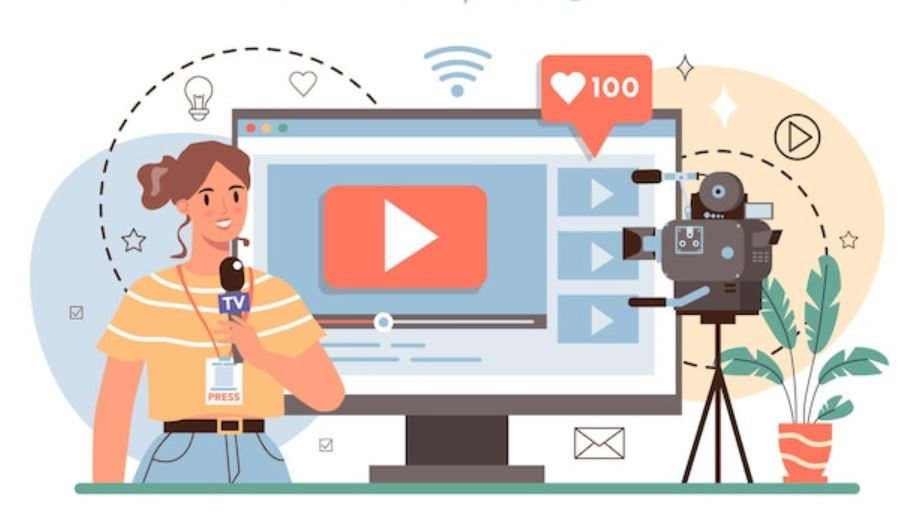
\includegraphics[height = 3cm, width = 5.8cm]{internet_novinarstvo.jpg}
  \end{center}
\end{frame}
\section{Zaključak}
\begin{frame}[fragile]\frametitle{Zaključak}
\transboxin
	\begin{itemize}	
		\item Popularizacija elektronskih tehnologija dovela je do promene u novinarstvu
        \item Internet novinarstvo biva lako prihvaćeno, pošto je adaptirano za krajnje korisnike
        \item Troškovi novinarstva na internetu nisu problem ni redakcijama ni čitaocima
        \item Kako je izveštavanje lakše i jeftinije - dobija se na slobodi medija, ali i gubi na kvalitetu informacija
	\end{itemize}
\end{frame}

\end{document}